\chapter{Entrada e Saída de teclado}

\chapterauthor{Matteo Cileneo Savan, Pedro Achilles Domingues Alves Pereira e Raul Yoshiyuki Komai}

%-------------------------------------------------------------------------------
\section{Descrição}
%-------------------------------------------------------------------------------

A entrada e saída (E/S) de dados formam a base da utilidade de qualquer sistema computacional. Sem esses subsistemas, a máquina torna-se incapaz de se comunicar com o mundo exterior. Um computador isolado é, na prática, apenas um amontoado de silício incapaz de resolver problemas reais. Neste contexto, esta seção detalha a implementação dos mecanismos de E/S, com foco na captura de dados via teclado e na saída visual em tela.

Tradicionalmente, a arquitetura dos dispositivos de E/S pode ser dividida em dois componentes principais:

\begin{description}
    \item[Componente Físico (ou Mecânico)] o dispositivo em si. É o hardware responsável por executar a operação de movimentar, exibir ou capturar os dados (as teclas de um teclado ou o painel de um monitor);
    \item[Componente Eletrônico] a controladora de dispositivo, que atua como interface entre o sistema principal e o componente físico. Na prática, ela expõe registradores para a comunicação com a CPU; a partir desses registradores, o sistema operacional torna-se capaz de enviar e receber dados, ler o estado do dispositivo, entre outras operações de controle.
\end{description}

O foco da implementação deste módulo é interagir com as controladoras de dispositivo por meio da criação de um \textit{driver} orientado a interrupções, eliminando a ineficiência da espera ocupada. Além disso, abordaremos o gerenciamento de \textit{buffers} de E/S e a implementação de interatividade com o usuário por meio de um \textit{shell} básico para a execução de comandos.

No ambiente do QEMU, a controladora simulada é a PrimeCell UART (PL011), que serve como base para a comunicação serial entre os dispositivos de E/S e o \textit{kernel}. É importante ressaltar que, neste cenário, não ocorre comunicação direta da UART com o teclado físico, tampouco com o monitor; toda essa operação é intermediada pelo próprio emulador QEMU \cite{ekasiswanto:qemu-uart}. Dessa forma, a plataforma expõe a interface necessária para a manipulação da controladora em baixo nível.


%-------------------------------------------------------------------------------
\section{Decisões de Arquitetura e Design}
%-------------------------------------------------------------------------------

O projeto visa tornar o sistema mais modular e facilitar futuras manutenções. Para refletir essa decisão estrutural, a implementação foi dividida em dois módulos: o arquivo \texttt{uart.c} concentra as funções de baixo nível da controladora UART, enquanto o arquivo \texttt{kstdio.c} fornece uma camada de abstração de mais alto nível, focada nas rotinas de E/S.

A respeito do gerenciamento temporário de dados na implementação da UART, optou-se pela utilização de um \textit{buffer} circular. Essa estrutura de dados foi escolhida por permitir o armazenamento e o consumo contínuo de fluxos de dados de maneira eficiente, operando sobre um espaço de memória estático e pré-alocado, além de apresentar uma implementação direta e de baixa complexidade.

Por fim, a arquitetura de comunicação com os dispositivos baseia-se estritamente em um sistema orientado a interrupções. Essa decisão evita o desperdício de recursos computacionais: o processador fica livre para executar outros processos ou tarefas do sistema, sendo notificado pelo hardware apenas quando ocorre, de fato, um evento (como o pressionamento de uma tecla), eliminando a ineficiência da espera ocupada.


%-------------------------------------------------------------------------------
\section{Detalhes da Implementação}
%-------------------------------------------------------------------------------

\subsection{Arquivos e Organização}

A base de código foi estruturada nos seguintes arquivos:

\begin{description}
    \item[\texttt{kstdio.c}] camada de abstração de alto nível sobre as funcionalidades da UART. Fornece um conjunto de rotinas de entrada e saída baseadas nas funções primitivas de \texttt{uart.c}, sendo amplamente utilizada no interpretador de comandos do sistema;
    \item[\texttt{main.c}] ponto de entrada do \textit{kernel}, coordena a inicialização geral do sistema;
    \item[\texttt{shell.c}] \textit{shell} interativo básico, capaz de ler, interpretar e executar comandos do usuário a partir do terminal do QEMU;
    \item[\texttt{uart.c}] encapsula toda a lógica de implementação do \textit{driver} da controladora UART emulada.
\end{description}

\subsection{Fluxo Simplificado de Execução}

Podemos dividir a execução das operações de E/S em dois fluxos principais: o de entrada (leitura) e o de saída (escrita). A seguir, detalhamos o caminho percorrido pelos dados ao atravessarem as diferentes camadas de abstração do sistema.

\subsubsection{Fluxo de Entrada}

Neste fluxo, ilustrado na Figura \ref{fig:fluxo-in}, o dado nasce no mundo físico e viaja até ser processado pelo sistema operacional. O usuário digita caracteres no teclado, que são capturados pelo terminal do QEMU e encaminhados para a UART emulada. Ao receber os dados, a UART aciona uma interrupção de hardware. O \textit{driver} intercepta essa interrupção, extrai os caracteres e os armazena de forma segura em um \textit{buffer} de entrada, disponibilizando-os para o \textit{shell} por meio de funções de leitura, como \texttt{uart\_getc()}.

\begin{figure}[htbp]
    \centering
    \resizebox{\textwidth}{!}{%
    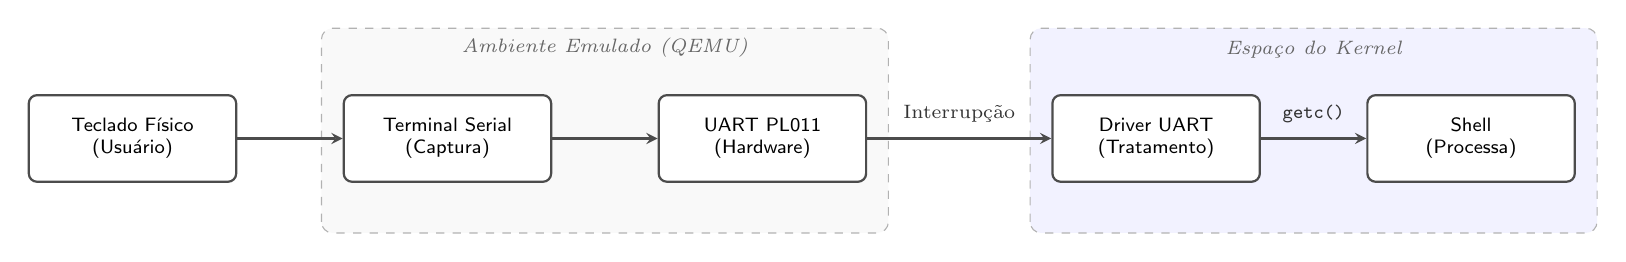
\begin{tikzpicture}[
        >=stealth,
        box/.style={
            rectangle, 
            draw=black!70, 
            thick, 
            rounded corners=3pt,
            minimum height=1.1cm,
            text width=2.4cm,
            align=center, 
            fill=white, 
            font=\scriptsize\sffamily
        },
        arrow/.style={
            ->, 
            thick, 
            draw=black!70
        }
    ]

    \filldraw[fill=gray!5, draw=black!30, dashed, rounded corners] (2.4, -1.2) rectangle (9.6, 1.4);
    \node[font=\itshape\scriptsize, text=black!60, anchor=south] at (6.0, 0.9) {Ambiente Emulado (QEMU)};

    \filldraw[fill=blue!5, draw=black!30, dashed, rounded corners] (11.4, -1.2) rectangle (18.6, 1.4);
    \node[font=\itshape\scriptsize, text=black!60, anchor=south] at (15.0, 0.9) {Espaço do Kernel};

    \node[box] (in_user)   at (0, 0)    {Teclado Físico\\(Usuário)};
    \node[box] (in_term)   at (4.0, 0)  {Terminal Serial\\(Captura)};
    \node[box] (in_uart)   at (8.0, 0)  {UART PL011\\(Hardware)};
    \node[box] (in_driver) at (13.0, 0) {Driver UART\\(Tratamento)};
    \node[box] (in_shell)  at (17.0, 0) {Shell\\(Processa)};

    \draw[arrow] (in_user) -- (in_term);
    \draw[arrow] (in_term) -- (in_uart);
    \draw[arrow] (in_uart) -- node[above=2pt, font=\scriptsize, text=black!80] {Interrupção} (in_driver);
    \draw[arrow] (in_driver) -- node[above=2pt, font=\scriptsize, text=black!80] {\texttt{getc()}} (in_shell);

    \end{tikzpicture}%
    }
    \caption{Pipeline do fluxo de entrada.}
    \label{fig:fluxo-in}
\end{figure}

\subsubsection{Fluxo de Saída}

No fluxo de saída, ilustrado na Figura \ref{fig:fluxo-out}, o caminho se inverte. O \textit{shell} utiliza funções da camada de abstração (como \texttt{kprintf()}, \texttt{kputs()} e \texttt{kputc()}) para enviar respostas ao \textit{driver} da UART. O \textit{driver}, por sua vez, escreve esses caracteres nos registradores da controladora emulada, que os transmite de volta ao QEMU para serem finalmente renderizados no terminal do usuário.

\begin{figure}[htbp]
    \centering
    \resizebox{\textwidth}{!}{%
    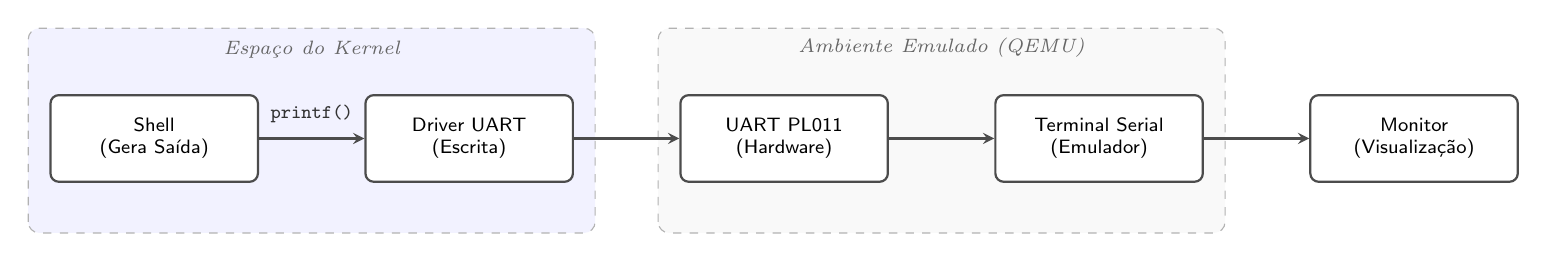
\begin{tikzpicture}[
        >=stealth,
        box/.style={
            rectangle, 
            draw=black!70, 
            thick, 
            rounded corners=3pt,
            minimum height=1.1cm,
            text width=2.4cm,
            align=center, 
            fill=white, 
            font=\scriptsize\sffamily
        },
        arrow/.style={
            ->, 
            thick, 
            draw=black!70
        }
    ]

    \filldraw[fill=blue!5, draw=black!30, dashed, rounded corners] (-1.6, -1.2) rectangle (5.6, 1.4);
    \node[font=\itshape\scriptsize, text=black!60, anchor=south] at (2.0, 0.9) {Espaço do Kernel};

    \filldraw[fill=gray!5, draw=black!30, dashed, rounded corners] (6.4, -1.2) rectangle (13.6, 1.4);
    \node[font=\itshape\scriptsize, text=black!60, anchor=south] at (10.0, 0.9) {Ambiente Emulado (QEMU)};

    \node[box] (out_shell)  at (0, 0)    {Shell\\(Gera Saída)};
    \node[box] (out_driver) at (4.0, 0)  {Driver UART\\(Escrita)};
    \node[box] (out_uart)   at (8.0, 0)  {UART PL011\\(Hardware)};
    \node[box] (out_term)   at (12.0, 0) {Terminal Serial\\(Emulador)};
    \node[box] (out_user)   at (16.0, 0) {Monitor\\(Visualização)};

    \draw[arrow] (out_shell) -- node[above=2pt, font=\scriptsize, text=black!80] {\texttt{printf()}} (out_driver);
    \draw[arrow] (out_driver) -- (out_uart);
    \draw[arrow] (out_uart) -- (out_term);
    \draw[arrow] (out_term) -- (out_user);

    \end{tikzpicture}%
    }
    \caption{Pipeline do fluxo de saída.}
    \label{fig:fluxo-out}
\end{figure}

\subsection{A Entrada de Dados via Teclado}

O teclado é um dispositivo de caractere. Diferentemente dos discos, que operam lendo e escrevendo dados em blocos de tamanho fixo, o teclado gera um fluxo sequencial e contínuo de caracteres independentes.

O driver implementado para gerenciar esse fluxo foi criado com base na especificação técnica da interface PL011 \cite{jankovic:qemu-uart-interface}. A comunicação em baixo nível é realizada mapeando na memória os principais registradores da controladora \cite{arm:summary-registers}, conforme detalhado na Tabela \ref{tab:uart-registradores}.


\begin{table}[htbp]
    \centering
    \renewcommand{\arraystretch}{1.3}
    \begin{tabular}{@{}llp{8cm}@{}}
        \hline
        \textbf{Registrador} & \textbf{Nome Completo} & \textbf{Descrição Funcional} \\
        \hline
        \texttt{UART0\_CR} & \textit{Control Register} & Habilita ou desabilita a UART, bem como as vias de transmissão (TX) e recepção (RX). \\
        \texttt{UART\_DR} & \textit{Data Register} & O \textit{kernel} lê deste endereço para obter dados recebidos e escreve nele para transmitir novos dados. \\
        \texttt{UART\_FR} & \textit{Flag Register} & Reflete o estado atual. Contém a flag \textbf{\texttt{RXFE}} (\textit{Receive FIFO Empty}), que indica se a fila de recepção está vazia. \\
        \texttt{UART0\_LCR\_H} & \textit{Line Control Register} & Controle de linha. Contém o bit \textbf{\texttt{FEN}} (\textit{FIFO Enable}) para habilitar as FIFOs de hardware. \\
        \texttt{UART0\_IMSC} & \textit{Interrupt Mask} & Define eventos geradores de interrupção. Destaque para as máscaras \textbf{\texttt{RXIM}} (recepção) e \textbf{\texttt{TXIM}} (transmissão). \\
        \texttt{UART0\_ICR} & \textit{Interrupt Clear} & Registrador de escrita; informa ao hardware que uma interrupção pendente foi devidamente tratada. \\
        \texttt{UART0\_MIS} & \textit{Masked Int. Status} & Registrador de leitura; indica exatamente quais interrupções (não mascaradas) estão pendentes no momento. \\
        \texttt{IBRD} e \texttt{FBRD} & \textit{Baud Rate Divisor} & Contêm, respectivamente, as partes inteira e fracionária do divisor para configurar a taxa de transmissão. \\
        \hline
    \end{tabular}
    \caption{Principais registradores da controladora UART PL011 utilizados na comunicação de E/S.}
    \label{tab:uart-registradores}
\end{table}

O \textit{kernel} efetiva o controle da UART lendo o \textit{status} e escrevendo configurações e dados diretamente nestes endereços mapeados.

\subsection{Inicialização da UART}
A rotina de inicialização ocorre por meio da chamada \texttt{uart\_init()}, que executa a seguinte sequência de passos, ilustrada na Figura \ref{fig:uart-init}.

\begin{figure}[htbp]
    \centering
    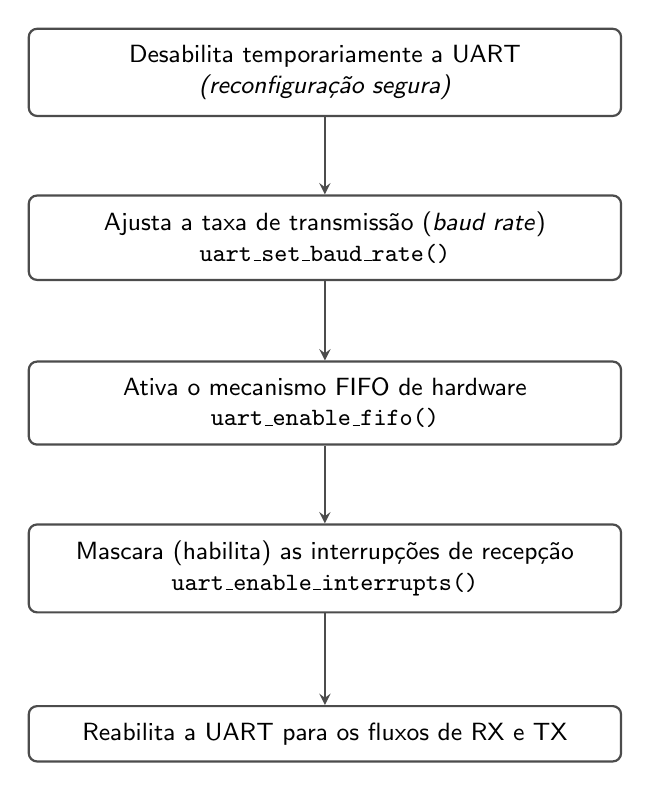
\begin{tikzpicture}[
        >=stealth,
        box/.style={
            rectangle,
            draw=black!70,
            thick,
            rounded corners=3pt,
            text width=7.1cm,
            align=center,
            fill=white,
            font=\small\sffamily,
            inner sep=6pt
        },
        arrow/.style={->, thick, draw=black!70}
    ]

    \node[box] (s1) at (0, 0)    {Desabilita temporariamente a UART\\\textit{(reconfiguração segura)}};
    \node[box] (s2) at (0, -2.1) {Ajusta a taxa de transmissão (\textit{baud rate})\\\texttt{uart\_set\_baud\_rate()}};
    \node[box] (s3) at (0, -4.2) {Ativa o mecanismo FIFO de hardware\\\texttt{uart\_enable\_fifo()}};
    \node[box] (s4) at (0, -6.3) {Mascara (habilita) as interrupções de recepção\\\texttt{uart\_enable\_interrupts()}};
    \node[box] (s5) at (0, -8.4) {Reabilita a UART para os fluxos de RX e TX};

    \draw[arrow] (s1) -- (s2);
    \draw[arrow] (s2) -- (s3);
    \draw[arrow] (s3) -- (s4);
    \draw[arrow] (s4) -- (s5);

    \end{tikzpicture}
    \caption{Sequência de inicialização da UART executada por \texttt{uart\_init()}.}
    \label{fig:uart-init}
\end{figure}

Ao final deste processo, o sistema encontra-se devidamente configurado para operar de forma assíncrona. Ao dispensar a espera ocupada (\textit{polling}), o \textit{kernel} delega ao controlador de interrupções a tarefa de notificá-lo apenas quando houver, de fato, novos caracteres a serem processados.
\subsection{Tratamento de Interrupções}

Sempre que um caractere é inserido no terminal do QEMU, a UART atualiza seu estado interno e levanta um sinal de interrupção (\textit{IRQ}). O controlador de interrupções da arquitetura intercepta esse sinal e desvia o fluxo de execução para a rotina de tratamento \texttt{uart\_irq\_handler(void)}, que realiza os seguintes passos lógicos:

\begin{enumerate}
    \item Verifica e valida a origem da interrupção lendo o registrador \texttt{UART0\_MIS};
    \item Confirma o tratamento do evento escrevendo no registrador de limpeza \texttt{UART0\_ICR};
    \item Consome os caracteres acumulados lendo diretamente o registrador \texttt{UART\_DR};
    \item Armazena em memória cada caractere recuperado chamando \texttt{uart\_buffer\_push()}, em um laço que se repete enquanto o hardware indicar que há dados válidos pendentes de leitura.
\end{enumerate}

\subsection{Gerenciamento de \textit{Buffer} Circular}

Como as velocidades de digitação e de processamento do \textit{kernel} são assimétricas, é necessário o armazenamento temporário dos dados recebidos. Para isso, estruturou-se uma fila circular, definida pelo tipo \texttt{ring\_buffer\_t}, cujos campos estão descritos na Tabela \ref{tab:ring-buffer-campos}.

\begin{table}[htbp]
    \centering
    \renewcommand{\arraystretch}{1.3}
    \begin{tabular}{@{}llp{7.5cm}@{}}
        \hline
        \textbf{Campo} & \textbf{Tipo} & \textbf{Descrição} \\
        \hline
        \texttt{buffer} & \texttt{char[]} & Vetor estático de caracteres em memória. \\
        \texttt{head} & \texttt{volatile uint32\_t} & Índice que rastreia a posição da próxima escrita. \\
        \texttt{tail} & \texttt{volatile uint32\_t} & Índice que rastreia a posição da próxima leitura. \\
        \hline
    \end{tabular}
    \caption{Campos da estrutura \texttt{ring\_buffer\_t}.}
    \label{tab:ring-buffer-campos}
\end{table}

A Figura \ref{fig:ring-buffer} ilustra o funcionamento do \textit{buffer} circular:

\begin{figure}[htbp]
    \centering
    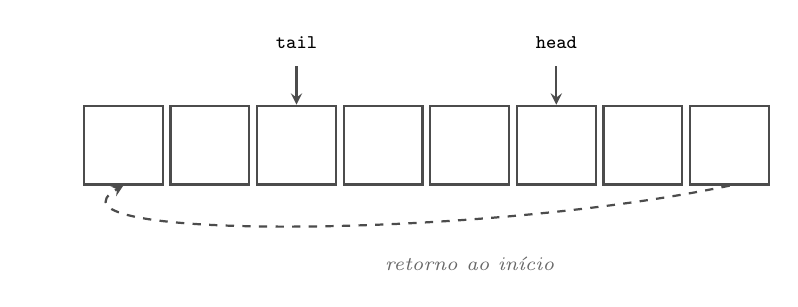
\begin{tikzpicture}[
        >=stealth,
        cell/.style={
            rectangle,
            draw=black!70,
            thick,
            minimum width=1cm,
            minimum height=1cm,
            font=\scriptsize\sffamily
        },
        ptr/.style={
            ->,
            thick,
            draw=black!70
        }
    ]

    \foreach \i in {0,...,7} {
        \node[cell] (c\i) at (\i*1.1, 0) {};
    }

    \node[font=\scriptsize\sffamily] at (2*1.1, 1.3) {\texttt{tail}};
    \draw[ptr] (2*1.1, 1.0) -- (c2.north);

    \node[font=\scriptsize\sffamily] at (5*1.1, 1.3) {\texttt{head}};
    \draw[ptr] (5*1.1, 1.0) -- (c5.north);

    \draw[ptr, dashed] (c7.south) .. controls (4*1.1, -1.2) and (-1.2, -1.2) .. (c0.south);
    \node[font=\itshape\scriptsize, text=black!60] at (4*1.1, -1.5) {retorno ao início};

    \end{tikzpicture}
    \caption{Os índices \texttt{head} (escrita) e \texttt{tail} (leitura) avançam de forma independente e retornam ao início do vetor ao atingir a última posição.}
    \label{fig:ring-buffer}
\end{figure}

A partir dessa estrutura central, instancia-se o objeto \texttt{rx\_buffer} (dedicado à recepção), cujas operações de inserção e remoção ocorrem estritamente por meio da interface de funções do \textit{driver}:

\begin{description}
    \item[\texttt{static int uart\_buffer\_push(char c)}] insere o caractere \texttt{c} na posição \texttt{head} e avança o índice circularmente. Retorna \texttt{1} em caso de sucesso (havendo espaço livre) e \texttt{0} caso contrário;
    \item[\texttt{static int uart\_buffer\_pop(char *ptr)}] consome um caractere da posição \texttt{tail}, gravando-o na região de memória apontada por \texttt{ptr}. Retorna \texttt{1} se houver dado disponível e \texttt{0} se o \textit{buffer} estiver vazio.
\end{description}

\subsection{A Saída de Dados no Monitor}

Assim como o teclado, o monitor de texto é gerido pelo sistema como um dispositivo de caractere. No ecossistema emulado deste projeto, as saídas textuais fluem pela mesma controladora UART (PL011). Toda vez que o \textit{kernel} escreve um caractere para exibição, o hardware transmite essa informação de volta pela interface serial, encarregando o QEMU de renderizar os caracteres no terminal de saída visual.

%-------------------------------------------------------------------------------
\section{Interface Pública (API)}
%-------------------------------------------------------------------------------

O subsistema de E/S disponibiliza duas \textit{APIs}: uma de baixo nível, voltada ao acoplamento direto com o hardware, e outra de alto nível, estruturada para abstrair operações comuns ao restante do \textit{kernel}.

\subsection{API da UART (Baixo Nível)}

Esta camada agrupa as funções primitivas de interação direta com a controladora UART PL011. Suas principais rotinas são:

\begin{description}
    \item[\texttt{void uart\_init(void)}]
    Inicializa e configura a UART PL011 para comunicação serial. Durante o processo, a controladora é temporariamente desabilitada, a taxa de transmissão (\textit{baud rate}) é ajustada, os \textit{buffers} FIFO são ativados e as interrupções de recepção são habilitadas. Ao término, a UART é reativada para operações de transmissão e recepção.

    \item[\texttt{void uart\_putc(char c)}]
    Transmite um único caractere \texttt{c} pela UART. Realiza automaticamente o tratamento do caractere de nova linha (\texttt{\textbackslash n}), convertendo-o para a sequência (\texttt{\textbackslash r\textbackslash n}) exigida por terminais seriais. Antes de efetuar a escrita no registrador de dados \texttt{UART\_DR}, a função aguarda a liberação de espaço no FIFO de transmissão.

    \item[\texttt{void uart\_puts(const char *str)}]
    Transmite uma sequência de caracteres apontada pelo parâmetro \texttt{str}, iterando sobre o vetor e enviando cada caractere sucessivamente por meio de \texttt{uart\_putc()}. Ao encontrar o caracter \textbackslash n, finaliza a transmissão.

    \item[\texttt{char uart\_getc(void)}]
    Função sem parâmetros que retorna um caractere que foi recebido e transmitido pela UART. Ela funciona como uma interface pública de leitura do que a UART transmite.

    \item[\texttt{void uart\_irq\_handler(void)}]
    Deve ser acionada diretamente pelo controlador de interrupções da arquitetura (GIC) sempre que o identificador de interrupção correspondente (\textit{IRQ ID} 33) for disparado pelo hardware da UART. Inicia uma rotina de tratamentos de interrupções de UART.
\end{description}

\subsection{API de Entrada e Saída do Kernel (\texttt{kstdio})}

Implementada sobre o módulo \texttt{kstdio.c}, esta interface fornece abstrações de mais alto nível para a comunicação textual e o processamento de comandos do sistema, encapsulando as complexidades da controladora UART. Suas funções compreendem:

\begin{description}
    \item[\texttt{void kstdio\_init(void)}]
    Inicializa o subsistema básico de entrada e saída do \textit{kernel}, acionando internamente a rotina de configuração da UART.

    \item[\texttt{void kputs(const char *str)}]
    Envia uma \textit{string} completa (recebida através de um ponteiro) para a saída serial, servindo como interface de alto nível para exibição de mensagens estáticas do \textit{kernel}.

    \item[\texttt{void kputc(char c)}]
    Envia um único caractere para a saída serial utilizando as rotinas de abstração de E/S.

    \item[\texttt{char kgetc(void)}]
    Função sem parâmetros que retorna um caractere que foi recebido e transmitido pela UART. Ela funciona como uma interface pública de leitura do que a UART transmite.

    \item[\texttt{char kgets(char *buf, int max\_len)}]
    Lê uma sequência de caracteres da entrada padrão até encontrar uma quebra de linha ou atingir o limite de comprimento especificado em \texttt{max\_len}, armazenando o resultado no vetor de destino \texttt{buf}.

    \item[\texttt{void kprintf(const char *format, ...)}]
    Implementação personalizada de formatação e impressão para o \textit{kernel}, inspirada na clássica função \texttt{printf()} da biblioteca padrão de C. Interpreta uma \textit{string} de formatação contendo especificadores, convertendo argumentos subsequentes para representação textual e direcionando-os à saída serial. Os especificadores de formato suportados estão listados na Tabela \ref{tab:kprintf-especificadores}.
\end{description}

\begin{table}[htbp]
    \centering
    \renewcommand{\arraystretch}{1.2}
    \begin{tabular}{@{}lp{9cm}@{}}
        \hline
        \textbf{Especificador} & \textbf{Descrição} \\
        \hline
        \texttt{\%c} & Caractere isolado \\
        \texttt{\%s} & Cadeia de caracteres (\textit{string}) \\
        \texttt{\%d} & Número inteiro decimal com sinal \\
        \texttt{\%u} & Número inteiro decimal sem sinal \\
        \texttt{\%x} & Representação em formato hexadecimal \\
        \texttt{\%\textit{n}f} & Número de ponto flutuante, formatado com \textit{n} casas decimais \\
        \texttt{\%\%} & Caractere literal de porcentagem (\%) \\
        \hline
    \end{tabular}
    \caption{Especificadores de formato suportados por \texttt{kprintf()}.}
    \label{tab:kprintf-especificadores}
\end{table}


%-------------------------------------------------------------------------------
\section{Testes e Verificação}
%-------------------------------------------------------------------------------

Para validar o funcionamento integrado de todo o subsistema de E/S, utilizou-se o interpretador de comandos (\textit{shell}) implementado no arquivo \texttt{shell.c}. O \textit{shell} provê uma interface de linha de comando simples para interação direta com o \textit{kernel} através da porta serial.

O fluxo de execução do \textit{shell} baseia-se em um laço contínuo que exibe um indicador visual (\textit{prompt} \texttt{\$}) e aguarda a entrada do usuário por meio da função \texttt{kgetc()}. Os caracteres digitados são armazenados temporariamente em um \textit{buffer} interno de comandos. Durante essa captura, o sistema trata dois caracteres especiais de controle, descritos na Tabela \ref{tab:shell-teclas}.

\begin{table}[htbp]
    \centering
    \renewcommand{\arraystretch}{1.2}
    \begin{tabular}{@{}lp{9cm}@{}}
        \hline
        \textbf{Tecla} & \textbf{Efeito} \\
        \hline
        \textit{Enter} & Finaliza a digitação da linha atual, sinalizando que o comando está pronto para o processamento. \\
        \textit{Backspace} & Remove o último caractere inserido, atualizando visualmente o terminal. \\
        \hline
    \end{tabular}
    \caption{Tratamento de teclas especiais pelo \textit{shell}.}
    \label{tab:shell-teclas}
\end{table}

Para garantir a interatividade, cada caractere imprimível digitado é imediatamente enviado de volta ao terminal através de \texttt{kputc()}, gerando o efeito de eco visual. Após a conclusão da linha, o \textit{shell} executa uma etapa de \textit{parser} (tokenização), que divide a entrada com base em espaços, preenchendo o vetor de argumentos \texttt{argv} e atualizando a contagem em \texttt{argc}.

O reconhecimento e a execução dos comandos são efetuados por meio de comparações de \textit{strings} utilizando a função \texttt{strcmp()}. O conjunto de comandos implementados, descrito na Tabela \ref{tab:shell-comandos}, permitiu testar exaustivamente as rotinas do sistema.

\begin{table}[htbp]
    \centering
    \renewcommand{\arraystretch}{1.3}
    \begin{tabular}{@{}lp{9cm}@{}}
        \hline
        \textbf{Comando} & \textbf{Função e Cobertura de Teste} \\
        \hline
        \texttt{help} & Exibe a listagem de comandos disponíveis, testando a capacidade de impressão de múltiplas linhas formatadas via \texttt{kprintf()}. \\
        \texttt{clear} & Limpa o terminal serial enviando a sequência de escape ANSI padrão (\texttt{\textbackslash033[2J\textbackslash033[H}) por meio da função \texttt{kputs()}. \\
        \texttt{echo} & Reproduz no terminal os argumentos subsequentes informados pelo usuário. Valida a leitura integrada do \textit{buffer}, a tokenização de \textit{strings} e a transmissão formatada de texto. \\
        \texttt{kprintf} & Executa uma bateria de testes da função de impressão formatada, validando a conversão e exibição de múltiplos especificadores (\texttt{\%s}, \texttt{\%c}, \texttt{\%d} e \texttt{\%x}). \\
        \hline
    \end{tabular}
    \caption{Comandos do \textit{shell} utilizados na verificação do subsistema de E/S.}
    \label{tab:shell-comandos}
\end{table}